\documentclass[12pt]{article}
\usepackage[utf8]{inputenc}
\usepackage{manfnt}
\usepackage{amsfonts}
\usepackage[margin=2cm]{geometry}
\usepackage[spanish]{babel}
\usepackage{graphicx}
\usepackage{tikz,pgfplots}
\usepackage{amsmath}
\usepackage{listings}

\begin{document}

% Meta informations
\title{Loki Text Adventure}
\author{Carlos Toledo Silva C-311\\
		    Ariel Alfonso Triana Pérez C-311}
\date{2021}

\makeatletter
\begin{titlepage}
\centering

\vspace{5cm}

{ \Huge \textbf{\@title}}

\vspace{1cm}

SEGUNDO PROYECTO DE PROGRAMACIÓN DECLARATIVA

\vspace{5cm}


\includegraphics[width=5cm]{./img/logo-matcom.jpg}

\vspace{5cm}

\textbf{Equipo de desarrollo:}

 \@author

\vspace{1cm}

\@date
\end{titlepage}
	

	
\section{Introducción}

En el siguiente documento se realizará la presentación de la aplicación \textbf{Loki Text Adventure}. Para esto se divide el resto del documento en secciones. En una primera sección se presenta la historia elaborada para la aplicación y en una posterior sección se explica cómo un usuario puede interactuar con la aplicación. Posteriormente se explica la implementación de la aplicación: estrategia que se siguió y descripción de los módulos implementados.

\section{Historia elaborada para la aplicación}

La historia que se narra en la aplicación está basada en la mitología nórdica. El usuario asume el papel de Loki: un dios embaucador de esta mitología y uno de los dioses más conocidos. El usuario, metido en el papel de Loki, tomará parte en una historia en la que pasará por diferentes aventuras y dificultades, donde las decisiones que tome y los actos que realice tendrán una influencia directa en la historia del mundo.

Válido aclarar que aunque la historia está basada en la mitología nórdica, muchos de los pasajes que en ella se narran no ocurren exactamente igual, ni siquiera en el orden correspondiente a como están realmente recogidos en la mitología. Otros muchos ni siquiera ocurrieron y son invención de los autores. De esta forma se ha adaptado la historia de Loki y otros personajes nórdicos para lograr hacer una historia entretenida y atractiva para el usuario.

La historia está compuesta de 3 capítulos, seguidos uno a continuación del otro. Es decir que para el usuario poder llegar el capítulo $i+1$ deberá haber triunfado en el capítulo $i$. Además cada capítulo cuenta con varios finales; en algunos el jugador sale triunfante pero en otros este podría acabar perdiendo la vida. Por esto motivo el jugador deberá escoger sabiamente, si es que quiere avanzar lo más posible.  

\section{Interacción entre el jugador y la aplicación}

Cuando se ejecuta la aplicación (ya compilada) lo primero que se ve es lo siguiente:

\begin{figure}[h]
	\begin{center}
		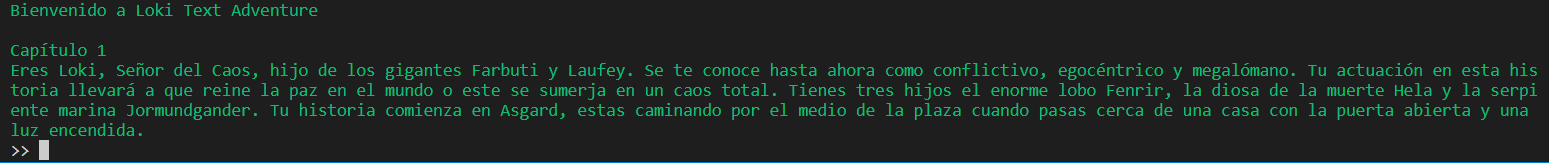
\includegraphics[width =15.0cm]{./img/Inicial.png}

        \caption{Inicio de la historia \label{fig:init}}
	\end{center}
\end{figure}

Aquí es donde comienza la historia. A medida que el personaje avance en la historia le irán saliendo texto similares a estos. Para poder avanzar el usuario deberá utilizar la información mostrada en cada uno de los textos y dar una respuesta lógica y bien escrita mediante alguna acción. Es importante señalar que las acciones se deben expresar mediante infinitivos: \textit{entrar}, \textit{aceptar}, \textit{hablar}, etc y que por supuesto estos se combinen con las otras palabras necesarias para elaborar una idea coherente. También es importante recalcar que, las acciones sobre el propio jugador deben ir seguidas del pronombre personal me; ejemplo: \textit{transformarme}, \textit{quedarme}, etc.

Por ejemplo, partiendo del texto inicial de la historia (Fig \ref{fig:init}) se puede hacer lo siguiente:

\begin{figure}[h]
	\begin{center}
		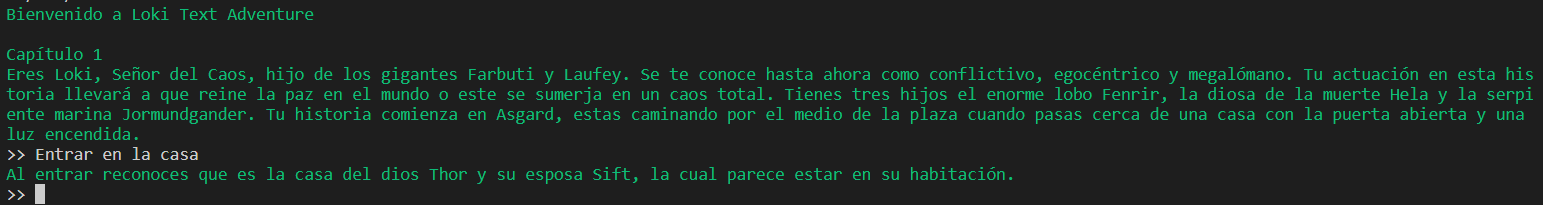
\includegraphics[width =15.0cm]{./img/Avance.png}

        \caption{Avance de la historia basado en la decisión del usuario}
	\end{center}
\end{figure}

Obsérvese cómo al escribir una acción lógica correctamente se ha avanzado en la historia. Si por el contrario se escribe una acción sin sentido o no escrita correctamente (ya sea por palabras mal escritas o falta de las mismas), la aplicación puede que no reconozca lo que el usuario quiere decir. Si ocurre este caso entonces se alertará con un mensaje y se volverá a imprimir el último texto de la historia. A continuación se muestra un ejemplo:

\begin{figure}[h]
	\begin{center}
		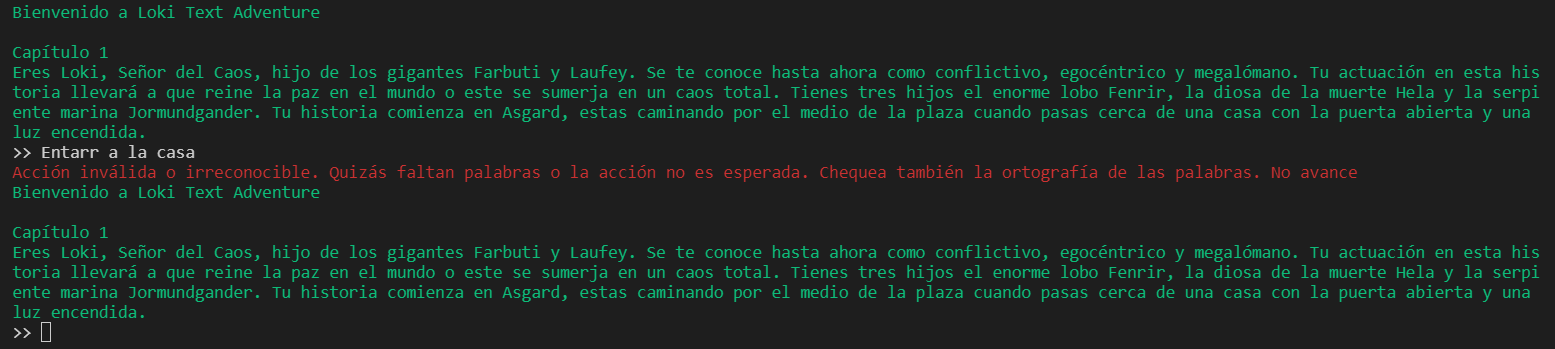
\includegraphics[width =15.0cm]{./img/No_avance.png}

        \caption{No se reconoce la decisión del jugador}
	\end{center}
\end{figure}

Fíjese que cuando salió el cartel por primera vez el usuario escribió mal la palabra ``Entrar'' y por este motivo la acción no se pudo reconocer. 

También durante el juego aparecerán situaciones en las que el usuario tendrá que escoger entre varias opciones. De esta forma la aplicación posibilita que el usuario pueda transitar por diferentes pasajes en base a sus decisiones. Cuan larga pueda ser la experiencia del jugador, también dependerá de las decisiones que tome. Una ``mala'' decisión, por decirlo de alguna forma, podría provocar que el usuario termine el juego antes de completar los 3 capítulos. Se muestra un ejemplo donde el usuario se enfrenta a una decisión: 

\begin{figure}[h]
	\begin{center}
		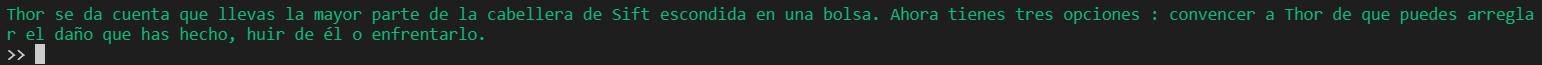
\includegraphics[width =15.0cm]{./img/Decision.png}

        \caption{Momento de trifurcación de la historia, en dependencia de la decisión del jugador}
	\end{center}
\end{figure}

En este caso el jugador podrá escoger entre convencer, hablar o enfrentar a Thor. En dependencia de lo que decida el usuario se moverá a uno u otro pasaje.

\section{Implementación}

En esta secci\'on se explica la estrategia de implementación de la aplicación, as\'i como los m\'odulos implementados y su funcionalidad.

\subsection{Estrategia de implementación}

Como toda historia, la presente está compuesta por diferentes pasajes. Por este motivo se define un tipo \verb|Passage| para representar los diferentes pasajes. Más adelante se verá como está implementado este tipo. En todo momento el jugador se va encontrar transitando en un determinado pasaje. Para cambiar de pasaje, lo cual provoca un avance en la historia, el jugador introduce una sentencia, a la cual se realiza un análisis para determinar si se cambia a algún otro pasaje o si la historia se mantiene en el mismo. Cuando se alcanza algún pasaje ``final'' la ejecución de la aplicación se detiene.

\subsection{Módulos implementados}

La implementación de la aplicación, para mejor organización y comprensión, está dividida en los siguientes módulos:

\begin{enumerate}
    \item[-] \textbf{Passages}: contiene la definición del tipo \verb|Passage|, y todos los pasajes de la historia.
    \item[-] \textbf{Synonyms}: contiene la definición del tipo \verb|Synonyms|, y todos los sinónimos utilizados en la historia.
    \item[-] \textbf{Functions}: contiene  la implementación de las funciones que permiten llevar el pasaje actual, el análisis de la entrada del usuario y el cambio o no de un pasaje a otro.
    \item[-] \textbf{Loki-Text-Adventure}: que apoyándose de los otros módulos permite el funcionamiento de la aplicación.
\end{enumerate}
 
A continuación se verán al detalle estos módulos y su funcionamiento.

\subsubsection{Módulo Passages}

Como se mencionó anteriormente, en este módulo está definido el tipo \verb|Passage| del cual veremos ahora su definición.

\begin{lstlisting}[language=Haskell, morekeywords={fix}]
data Passage = Passage {
        pid :: Int, 
        text :: String, 
        keywords :: [String], 
        nextPossiblePassages :: [Passage]
    }
\end{lstlisting}


El entero \verb|pid| se utiliza para comparar pasajes de una forma eficiente. La cadena \verb|text| es el texto correspondiente a un pasaje. Esto es lo que se imprime en pantalla cuando se llega a dicho pasaje. La lista de Passage \verb|nextPossiblePassages| son los pasajes a los cuales se puede avanzar a partir del pasaje actual. La lista de cadenas de texto \verb|keywords| son las palabras que debe teclear el usuario (o algunas que sean sinónimos de estas o que transmitan una idea similar) que permiten a partir de un pasaje específico alcanzar el pasaje con esas keywords. O sea, si  el usuario se encuentra en el pasaje $i$ y en la lista \verb|nextPossiblePassages| del pasaje $i$ se encuentra el pasaje $j$, para que el usuarió pueda pasar del pasaje $i$ al pasaje $j$ deberá teclear las palabras que aparecen en la lista \verb|keywords| del pasaje $j$ (o algunas que sean sinónimos de estas o que transmitan una idea similar). De esta forma es que ocurre el cambio entre pasajes.

De la forma antes descrita, aparecen además definidos todos los pasajes de la historia. El pasaje inicial es el único que tiene su lista \verb|keywords| vacía pues este no se alcanza desde ningún otro pasaje. Los pasajes finales, o sea los que no permitan avanzar al jugador más allá de ellos, se caracterizan porque su lista de pasajes \verb|nextPossiblePassages|  es una lista vacía.

\subsubsection{Módulo Synonyms}

Como se había mencionado al inicio de esta sección, el módulo \textbf{Synonyms} contiene la definición de un tipo del mismo nombre que el módulo. Esta definición se presenta a continuación:

\begin{lstlisting}[language=Haskell, morekeywords={fix}]
data Synonyms = Synonyms { 
        key :: String, 
        sym :: [String]
    } deriving (Eq,Show)
\end{lstlisting}

Con este tipo se puede definir un ``diccionario de sinónimos'', donde la cadena de texto \verb|key| representa la palabra de la cual se desean conocer los sinónimos y la lista de cadenas \verb|sym| representa los sinónimos de esa palabra.

Utilizando este tipo se precisó un diccionario de sinónimos para la historia donde los campos \verb|key| son las \verb|keywords| del tipo \verb|Passage| en cuestión, y \verb|sym| representa el todas las palabras que pueden ser utilizadas en lugar de \verb|key|. Todos estos sinónimos se fijan en la lista \verb|allSynonyms|. 

\subsubsection{Módulo Functions}

En este módulo se encuentran definidas las funciones que permiten el correcto funcionamiento de la aplicación. Este módulo depende de los anteriores para su correcto funcionamiento.

La función \verb|actualPassage| permite la creación de una variable global en la que se guardará en todo momento el pasaje en el cual se encuentra la historia. 

La función \verb|changePassage| recibe como parámetro un \verb|Passage| y lo que hace es definir al pasaje actual como el pasaje que se le pasa de entrada.

La función \verb|obtainPassage| se utiliza para poder obtener el pasaje actual en el que se encuentra la historia.

La función \verb|next| se utiliza para obtener el siguiente pasaje de la historia dado el pasaje actual y la entrada del usuario. El funcionamiento es el siguiente se construye una lista que contiene los pasajes que son ``descendientes directos'' del pasaje actual en la historia, cuyas \verb|keywords| están de forma exacta o a través de sinónimos en la entrada del usuario. Si esta lista no contiene elementos entonces se devuelve el pasaje actual, pues la decisión del usuario no se corresponde con las opciones disponibles. Si la lista contiene elementos esto quiere decir que con esa entrada se puede alcanzar cualquiera de los pasajes en la lista por tanto se devuelve el primer elemento. De esta forma se garantiza que siempre se devuelva un solo pasaje incluso cuando el usuario no fue preciso con lo que quer\'ia hacer. La función anterior utiliza  \verb|identifyKeywords| que realiza el procedimiento de chequear si la entrada del usuario contiene las \verb|keywords| del pasaje o sus sinónimos. Para esto utiliza \verb|getSym| que devuelve todos los sinónimos de cada \verb|keywords| del pasaje, y además utiliza \verb|find| que devuelve un booleano indicando si una cadena de texto está en una lista de cadenas de texto.


\subsubsection{Módulo Loki-Text-Adventure}

Este es el m\'odulo principal de la aplicaci\'on. En este m\'odulo primero tenemos dos funciones \verb|isWindows| y \verb|setEncoding|. La primera la utilizamos para saber si la aplicaci\'on se est\'a ejecutando en Windows o no. La segunda se utiliza para cambiar el formato de codificaci\'on de caracteres a UTF-8 en caso de que no estemos en Windows. Esto lo hacemos porque nos paso que uno de nostros program\'o en Windows 10 y el otro en Ubuntu 18.04 y si no cambiamos el formato de codificaci\'on de caracteres en Ubuntu la aplicaci\'on no reconoc\'ia los caracteres del Español como las tildes y la ñ. Sin embargo si cambiamos esta codificaci\'on en Windows ocurr\'ia entonces que dichos caracteres no se reconoc\'ian y al no cambiarlo si lo hac\'ian. Por tanto se opt\'o por comprobar si se estaba ejecutando la aplicaci\'on en Windows para cambiar o no la configuraci\'on de codificaci\'on de caracteres.

Entonces tenemos tambi\'en la funci\'on \verb|main|, la principal de toda la aplicaci\'on. En esta funci\'on primeramente en dependencia del sistema operativo se cambia o no la configuraci\'on de codificaci\'on de caracteres. Luego se obtiene el pasaje actual mediante la funci\'on \verb|obtainPassage|, se guarda en la variable \verb|passage| y de este se imprime su texto correspondiente. Luego, a menos que este sea un pasaje final, se espera a que el usuario propicie una entrada. En caso de ser un pasaje final se termina la ejecuci\'on. Entonces si la entrada propiciada por el usuario es \verb|salir| se detiene la ejecuci\'on; en cualquier otro caso se pasa a obtener el siguiente pasaje mediante la funci\'on \verb|next| y se guarda en la variable \verb|auxPassage|. Entonces comprobamos si el pasaje actual y el hallado por la funci\'on coinciden. De ser as\'i es porque el usuario no tecleo una entrada que permitiera el avance a un nuevo pasaje y en este caso se le escribe un mensaje de advertencia con las posibles causas del fracaso en el avance y se llama al m\'etodo \verb|main|. En caso de que no coincidan, es porque hubo un avance y por tanto se actualiza el estado actual mediante la funci\'on \verb|changePassage| utilizando como par\'ametro \verb|auxPassage|. Luego de esto llamamos al m\'etodo \verb|main|. Obs\'ervese que la aplicaci\'on solo termina su ejecuci\'on si se alcanza un pasaje final o el usuario tecla la palabra \verb|salir|.   

\end{document}